\documentclass[11pt]{mpreport}
\usepackage[utf8]{inputenc}
\usepackage[T1]{fontenc}
\usepackage[scaled=0.85]{helvet}
\usepackage[colorlinks=true,linkcolor=black,citecolor=black, urlcolor=black]{hyperref}
\usepackage{microtype}
\usepackage{fancyhdr}
\usepackage{graphicx}
\usepackage{palatino}
\usepackage{listings}
\usepackage{appendix}
\usepackage{remreset}
\usepackage{qtree}
\usepackage{wrapfig}
\usepackage{array}
\usepackage{multirow}
\usepackage{amsmath}
\usepackage{amssymb}
\usepackage{color}
\usepackage{hyperref}
\usepackage{caption}
\usepackage{subcaption}
\usepackage{float}

\makeatletter
\@removefromreset{footnote}{chapter}
\makeatother



\setlength{\headheight}{15.2pt}
\pagestyle{fancy}
\fancyhead[RO]{\thepage}
\fancyhead[LO]{}
\fancyfoot{}

\newcommand{\TODO}[1]{\hspace{-1.45cm}\textcolor{red}{ \textbf{TODO: #1}}}
\newcommand{\ITODO}[1]{\textcolor{red}{ \textbf{TODO: #1}}}





\definecolor{orange}{rgb}{1,.49,.18}
\definecolor{darkgreen}{rgb}{0,.66,.0}
\definecolor{mypurple}{rgb}{.76,0,.83}
\newcommand{\var}[1]{{\color{orange} \textbf{#1}}}
\newcommand{\autovar}[1]{{\color{darkgreen} \textbf{#1}}}
\newcommand{\conj}[1]{{\color{mypurple} \textbf{#1}}}



\fancypagestyle{plain}{%
   \fancyhf{}%
   \fancyhead[C]{} %Kapitelname ausblenden

   \renewcommand{\headrulewidth}{0.0pt} %obere Linie ausblenden
   \fancyfoot[C]{\thepage}
}

\setcounter{secnumdepth}{2} 




\begin{document}
\lstset{language=Java, basicstyle=\footnotesize}

\renewcommand{\thepage}{\roman{page}}
\newcommand{\monthword}[1]{\ifcase#1\or January\or February\or March\or April\or
                                        May\or June\or July\or August\or
                                        September\or October\or November\or December\fi} 

  \begin{titlepage}
    \def\fakultaet{Faculty of Mathematics and Computer Science}
    \par
    \unitlength1mm
    \begin{picture}(-2,12)
      \put(-1,11){\rule{165mm}{1mm}}
      \put(-4,-17){
        \parbox[b]{130mm}{
          \raggedleft{
            \fontsize{14}{18}\selectfont
            SAARLAND UNIVERSITY\\
            ~\\
            \fontfamily{ptm}\fontsize{12}{14}\selectfont \fakultaet\\
           Department of Computer Science\\
            Related Work Summary\\
          }
        }
      }
      \put(130,-20){
\includegraphics[height=30mm]{uds}}
      \put(-1,-20){\rule{130mm}{.25mm}}
    \end{picture}
    
    
    \vspace{6cm}
	\hspace{3cm}\parbox[b]{150mm}{
    \begin{flushleft}
      \sffamily\Huge
	Steadily Recalibration of Head Mounted\\
  Eye Trackers using Optical Flow\\
  and Attention\\
~\\
     
      
    \end{flushleft}

}
      \vfill
\hspace{3cm}\parbox[b]{120mm}{
      \sffamily \Huge
      Syed Mehran Hussain\\
      \Large
     \monthword{\month} \the\year
}

    \hspace{-5cm}
    \rule{8cm}{2.25mm}
    \hspace{-5cm}
    \rule{18cm}{.25mm}
  \end{titlepage}



\pagestyle{empty}

\vspace*{0.5cm}
\textbf{Advisor:}\\
Christian Lander\\
German Research Center for Artificial Intelligence\\
Saarland Informatics Campus\\
Saarbrücken, Germany

\vspace{4.5cm}
Started on 15/12/2017\\
%Status: \textit{in progress}
%Handed in on 02/02/2018


\vspace{4.5cm}


\vspace{3cm}
Saarland University\\
Faculty of Natural Sciences and Technology I\\
Department of Computer Science\\
Campus - Building E1.1\\
66123 Saarbrücken\\
Germany\\




\clearpage

\begingroup
  \pagestyle{plain}

\setcounter{tocdepth}{3}
  \addtocontents{toc}{\protect\thispagestyle{plain}}
  \addtocontents{toc}{\protect\vspace{-.45cm}}
  \tableofcontents
  \clearpage
\endgroup 

\pagestyle{fancy}
\setcounter{page}{1}
\renewcommand{\thepage}{\arabic{page}}


% \setcounter{secnumdepth}{3}


\section{Introduction}

In contrast to the current work on remote-based eye trackers, we will use head-mounted eye trackers, pupil centre corneal reflection (PCCR) and smooth pursuit to tackle the calibration problem. The smooth pursuit calibration is based on the smooth pursuit eye movement which we naturally perform when we follow a moving object with our eyes.\\

In our approach, we are looking to incorporate scenario of head movements during pursuit calibration. The user head movement during pursuit calibration can be detected using various methods, and can also be combined with eye tracking procedure. Satoh et al. \cite{7} proposed a head tracking method that uses a gyroscope mounted on a head-mounted-device and a fixed bird's-eye view camera responsible for observing the head-mounted-device from a third-person viewpoint.

\section{Eye Physiology}

Human eye is an organ of vision. Our eye movements are reflective to our emotional states and cognitive processes.

\subsection{Fixation}

These movements generally measured by fixations which is where a user looks. A fixation is an instant where the eyes are relatively stay still \cite{15}. Fixation is not a real movement by itself \cite{13}, as it describes the state of resting the gaze at a specific target within the central vision for a certain amount of time, typically around 200-300 milliseconds (ms). Fixation can be measured with frequency and the length of time looking at the content. Fixations can be interpreted in different ways depending on the context. A study \cite{24} suggested that a higher number of fixations during a task, such as looking at a web page, shows more processing time needed or there is great difficulty identifying the target object. Therefore, longer fixation duration (or clusters of fixations) may indicate strong interest and engagement with the target.

\subsection{Saccades}

After fixation, there are saccades which define rapid eye movements between fixations. Saccades are fast, hop from one state to another movements of the eye to refocus it between two consecutive fixations, with a duration of 30-80 ms \cite{13}. Another eye movement is smooth pursuit and is performed to closely tracks a moving object by steadily matching its velocity with the eye (e.g. looking at a moving car).


\begin{figure}[!hbt]
  \centering
  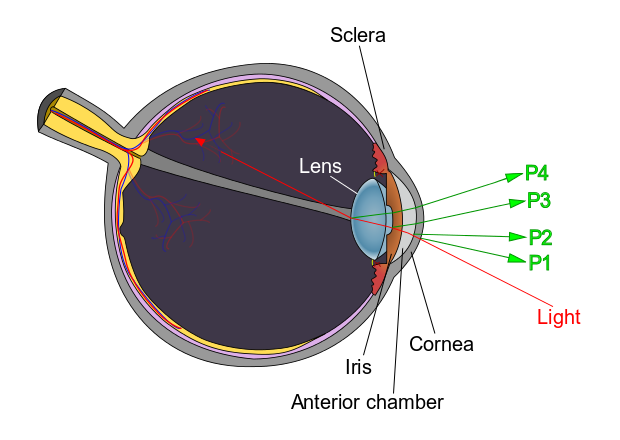
\includegraphics[width=4in,height=3in]{pimage.png}
  \caption{Diagram of light and four Purkinje images.}
  \label{pimage}
\end{figure}

\section{Eye Tracking and Gaze Estimation}

Today there are three main strategies used to perform eye tracking and gaze estimation. First, the electro-oculography (EOG) method is based on placing electrodes around the eye to measure the skin potentials. The generated electric signal is detected using two pairs of electrodes \cite{3}. Second, the scleral search coil method is based on using a small coil that is embedded into a contact lens. It measures the voltage caused by an external electro magnetic field \cite{25}. Third, the Camera-based (video based) methods which use the images of an eye to detect its characteristics in combination with images of the field of view to realize gaze estimation \cite{13}. The camera-based method is frequently used today on a head-mounted or remote system. Where cameras are mounted on the head or placed in the environment accordingly.\\

Gaze estimation is the primary task of eye trackers. Gaze can be defined as either the gaze direction or the point of regard (PoR). A person’s gaze is usually determined by the head pose including both position and orientation with the eyeball rotation. The gaze changes if at least one of the two (head pose or eyeball rotation) changes its value. Head movements are necessary to achieve very accurate gaze estimation. Head movements can be detected via additional hardware (e.g., tracking the head, as done with remote trackers), or integrating them directly into the method being used.\\

Various camera based eye trackers use light reflection points on the cornea to estimate the gaze direction, a technique known as pupil centre corneal reflection (PCCR) \cite{1}. Another name for eye images containing corneal reflection points is Purkinje Image \cite{2}. The first Purkinje image (P1) or corneal reflection is often called a glint as shown in Figure \ref{pimage}.

When using this approach, the vector between the center of the pupil and the corneal reflections is used to compute the gaze direction \cite{3}. These measurements, such as pupil position, limbus position, relative position of Purkinje images, and so on, must be translated to eye orientation. A calibration procedure is needed to compute the mapping between the measurements and the eye orientation before using the eye tracker. Unfortunately, this process of calibration is of poor usability and often regarded as tedious and difficult \cite{4}. 


\subsection{hEYEbrid: A Hybrid Approach for Mobile Calibration-free Gaze Estimation}

In Christian Lander, et.al \cite{13} paper, hEYEbrid: A Hybrid Approach for Mobile Calibration-free Gaze Estimation, an approach named hEYEbrid is proposed. This approach deals with calibration-free and very accurate gaze estimation in pervasive settings. This appraoch is different to existing systems as it combines the images from an infrared eye and a corneal camera in a hybrid approach and works without any prior user calibration. Therefore, the accuracy of this approach is robust against calibration drifts. The method is integrated into Pupil Lab’s \cite{29} open-source eyeracking framework, by adding a corneal camera to the head-mounted device and developing plugins for the capture and player software.

\begin{figure}[!hbt]
  \centering
  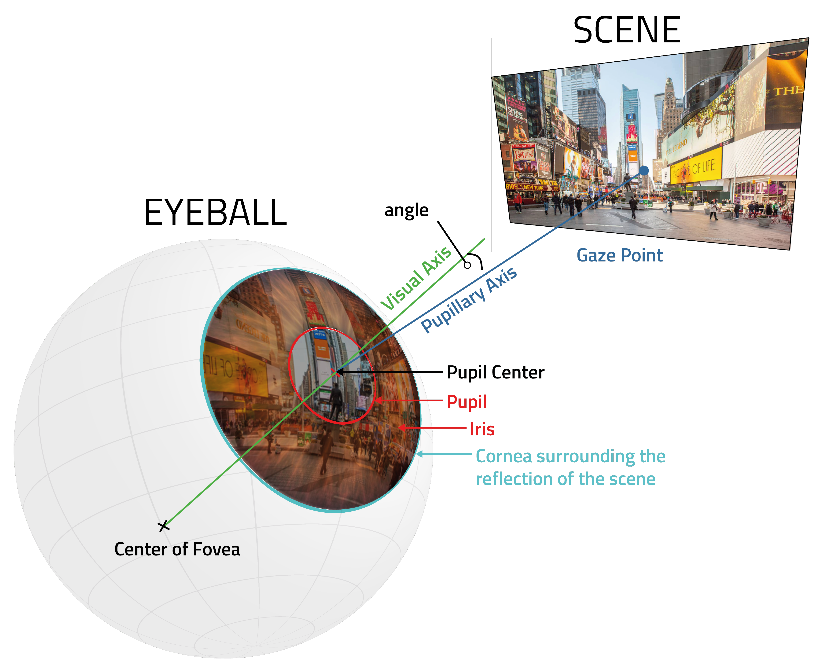
\includegraphics[width=3in,height=2.5in]{lander1.png}
  \caption{Basic idea of hEYEbrid to use the pupil center in the corneal image (i.e. the environment reflected on the human eye) as the gaze point in the actual scene.}
  \label{lander1}
\end{figure}


While proposing this appraoch, authors have conducted a user study in which they used a mobile setup to evaluate hEYEbrid’s gaze estimation accuracy against a state-of-the-art Pupil Labs eye tracker and 3C-hEYEbrid. Where 3C-hEYEbrid is an extended version of hEYEbrid which uses the scene camera as additional image information.


\begin{figure}[!hbt]
  \centering
  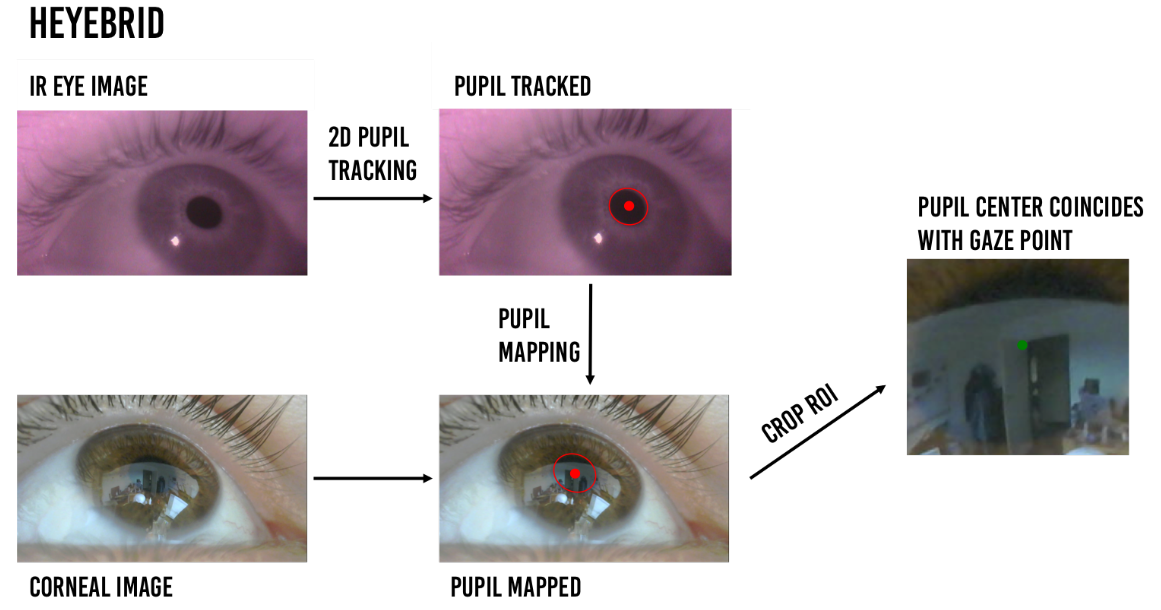
\includegraphics[width=4.5in,height=2in]{lander2.png}
  \caption{Basic processing pipeline of hEYEbrid, which combines infrared eye and corneal images. The pupil is tracked in the IR image and mapped onto the corneal image to finally crop the reflection within the pupil. The mapped pupil center coincides with the gaze point.}
  \label{lander2}
\end{figure}


Relating to the prospective work, the approach presented in this paper performs better than the well-established Pupil Labs eye tracker. It also compares well to existing approaches based on corneal imaging. The results are relatively promising, because of its robustness, and it defines the potential to implement mobile gaze-based interaction in everyday life settings.


\subsection{Eye gaze tracking techniques for interactive applications}

In Carlos H. Morimoto, et.al \cite{15} paper, Eye gaze tracking techniques for interactive applications, authors have described the state-of-the-art remote eye gaze trackers (REGTs), and showed that two of the major usability concerns of current REGT technology. 

\begin{figure}[!hbt]
  \begin{subfigure}{.5\textwidth}
    \centering
    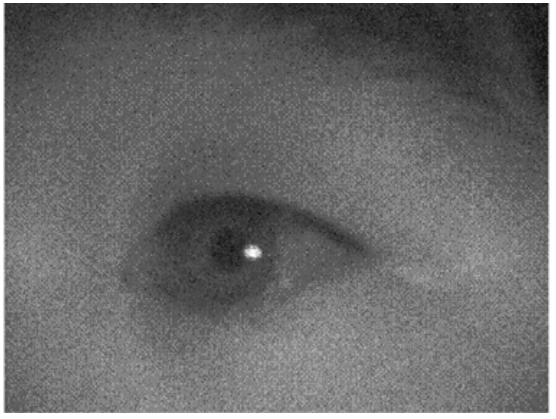
\includegraphics[width=2in,height=1.7in]{carlos.png}
    \caption{Dark}
    \label{carlos1}
  \end{subfigure}
  \begin{subfigure}{.5\textwidth}
    \centering
    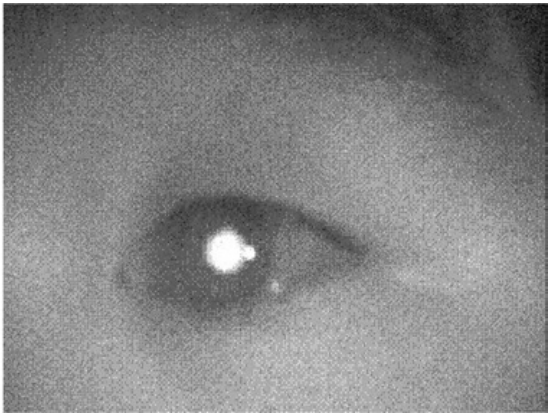
\includegraphics[width=2in,height=1.7in]{carlos2.png}
    \caption{Bright}
    \label{carlos2}
  \end{subfigure}
  \caption{Dark and bright pupil images.}
\end{figure}

The constant system calibration and a relatively limited head motion have requisits that are being answered by the current generation of REGTs.

\begin{figure}[!hbt]
  \centering
  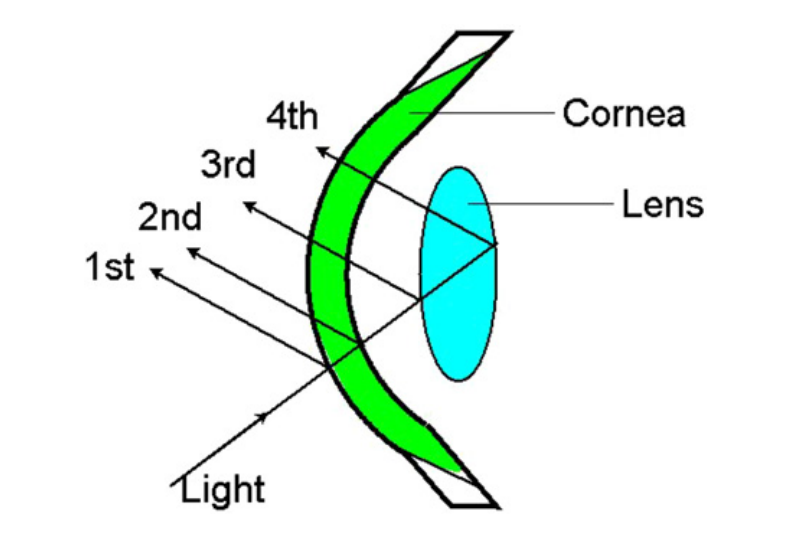
\includegraphics[width=3in,height=2in]{carlos3.png}
  \caption{Purkinje images.}
  \label{carlos3}
\end{figure}

The correlation between this paper and the prospective work is of usability concerns on remote eye gaze trackers. We will be using head-mounted eye trackers but the conventional methods in this paper can be used for eye gaze tracking in head-mounted eye trackers as well. They have focussed the main discussion of paper on the pupil-corneal reflection technique. In this paper, authors have showed that eye trackers were laboratory instruments, and therefore, many intrusive techniques could be tolerated. However, the development of general computer eye-aware computer applications need new usability requirements which must be satisfied beforehand.

\subsection{In the Eye of the Beholder: A Survey of Models for Eyes and Gaze}

In Dan Witzner Hansen, et.al \cite{16} paper, In the Eye of the Beholder: A Survey of Models for Eyes and Gaze, authors have introduced a brief review about generalizing eye tracking systems from different point of views. These point of views span over different methods of detecting and tracking eye images to computational models of eyes for gaze estimation and gaze-based applications. However for eye detection and tracking method, authors have discussed various techniques using different properties of the eyes including appearance, shape, motion, or some combination.

\begin{figure}[!hbt]
  \centering
  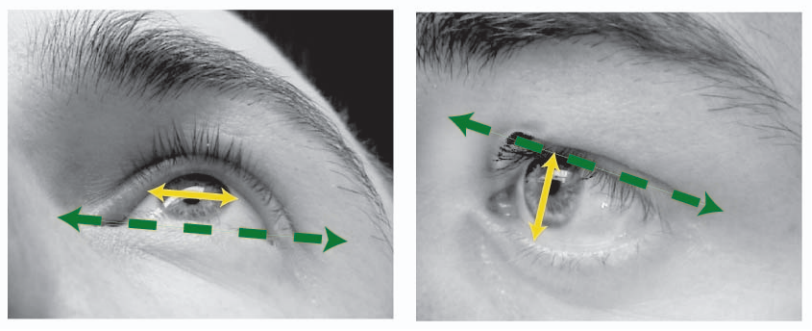
\includegraphics[width=4in,height=1.5in]{danWitzer.png}
  \caption{The shape of the eye may change drastically when viewed from different angles. For example, the eyelids may appear straight from one view but highly curved from another. The iris contour also changes with viewing angle. The dashed lines indicate when the eyelids appear straight, while the solid yellow lines represent the major axis of the iris ellipse.}
  \label{danwitzner}
\end{figure}

\begin{figure}[!hbt]
  \centering
  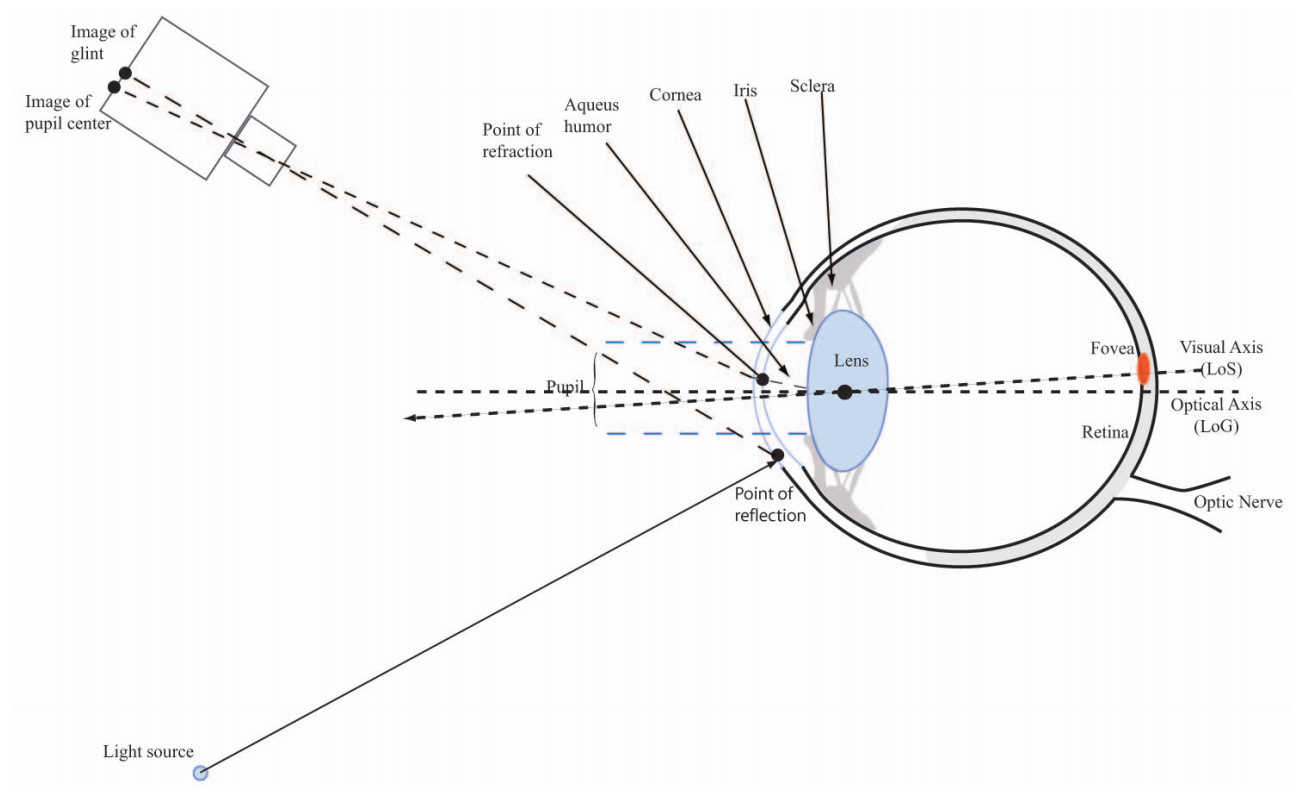
\includegraphics[width=4in,height=2.5in]{danWitzer2.png}
  \caption{General model of the structures of the human eye, light, light sources, and projections.}
  \label{danwitzner2}
\end{figure}


Techniques that had been surveyed in this paper mainly focus in the areas of eye detection and gaze tracking. Furthermore, most of these techniques can also be useful for detection and tracking of other objects e.g., faces. Even though describing the structure of the eye is relatively simple than other comparable objects but the complexities in its appearance make the eye a challenging task to analyse. In this and related papers new models has already been spawned by unique and sound problems from Eye and gaze tracking with their applications. \\

Regarding prospective work, these models are can be influencing beyond eye tracking. Eyes could also be seen as a primary case for prospective models of image analysis, geometry, and machine learning because of the inherent challenging properties of the eye as a trackable subject. For this reason, methods in this paper regarding eye tracker development is of increasing interest to a wide variety of our prospective work in making gaze estimation.

\subsection{Eye Tracking and Head Movement Detection: A State-of-Art Survey}

The Amer Al-Rahayfeh, et.al \cite{3} survey from recent years illustrates the state-of-the-art eye trackers and their corresponding usages and background. Eye tracking technology has progressed significantly. In fact, in the last few years eye trackers have become commercially available for mobile devices. Although the eye tracking technology for remote devices is still evolving compared to eye tracking on desktops and latptops, the data collection of today are now precise and reliable enough to provide meaningful insights.

Current state-of-the-art eye trackers can be shown in three classes: Sensor-Based (EOG), Computer-Vision-Based (CR, IR), Smartphone based.

Sensor-Based eye trackers process eye movements using electric potentials. These electric potentials are measured with electrodes placed around the eyes. This electric signal detected using two pairs of electrodes is known as electrooculogram (EOG). When the eyes are in their origin state, the electrodes measure a steady electric potential field. If the eyes move towards the periphery, the retina approaches one electrode and the cornea approaches the other. This changes the orientation of the dipole and results in a change in the measured EOG signal. Eye movement can be tracked by analyzing the changes in the EOG signal \cite{9}.


The most widely used current eye tracking devices are computer-vision-based. In this type of eye trackers, a camera focuses on one or both eyes and records eye movement as the viewer looks at some kind of stimulus. Most modern eye-trackers use the center of the pupil and (near) infrared non-collimated light to create corneal reflections (CR). The vector between the pupil center and the corneal reflections can be used to compute the point of regard on surface or the gaze direction. 

There are two types of (near) infrared (also known as active light) eye-tracking methods. One is bright-pupil and the other dark-pupil method \cite{10}. The difference between them is based on the location of the illumination source with respect to the optics. If the illumination is coaxial with the optical path, then the eye acts as a retroreflector where the light reflects off the retina creating a bright pupil effect similar to red eye. If the illumination source is offset from the optical path, then the pupil appears dark because the retroreflection from the retina is directed away from the camera \cite{10}.


Smarthphone based eye trackers have emerged with the advancement in technology. It has now become possible to use smartphones and tablets as eye trackers \cite{11}\cite{12}. As shown in He et al's paper \cite{14}, the front camera of a smartphone can be used to capture images of users, and then the OpenCV computer vision framework can be used to detect face, eye, and eye blinks.\\

This paper gives an introductory view on prospective work. The knowledge of current state-of-the-art eye trackers are important to understand before making strategies and methods to solve the calibration problem. Therefore, this paper gives rather strong introduction in the background and current eye trackers and head movement detection methods.

\subsection{I see what you see: Point of Gaze Estimation from Corneal Images}

In Christian Nitschke, et.al \cite{20} paper, I see what you see: Point of Gaze Estimation from Corneal Images, authors introduced the first Eye-gaze tracking approach that estimates the point of gaze  with respect to the reflected scene in an eye image. There basically two main contributions mentioned in the paper, one is the concept of direct point of gaze estimation, and second is a closed-form solution for the gazereflection point, including compensation for the individual offset between optical and visual axis.\\

The approach presented in this paper solves two major problems regarding existing methods. One is the calibration of relationship between eye camera and scene. Second is a parallax error that occurs under varying scene depth. There are respective practical advantages of these methods which includes reduced intrusiveness and complexity, and the support for flexible dynamic setups, non-planar and bright outdoor scenes. As these practical advantages enable various applications to work smoothly. These applications include eye-gaze tracking with infants, elderly and disabled, wearable eye-gaze tracking with ubiquitous cameras and AR-HMDs, and remote eye-gaze tracking, surveillance and forensics.

\begin{figure}[!hbt]
  \centering
  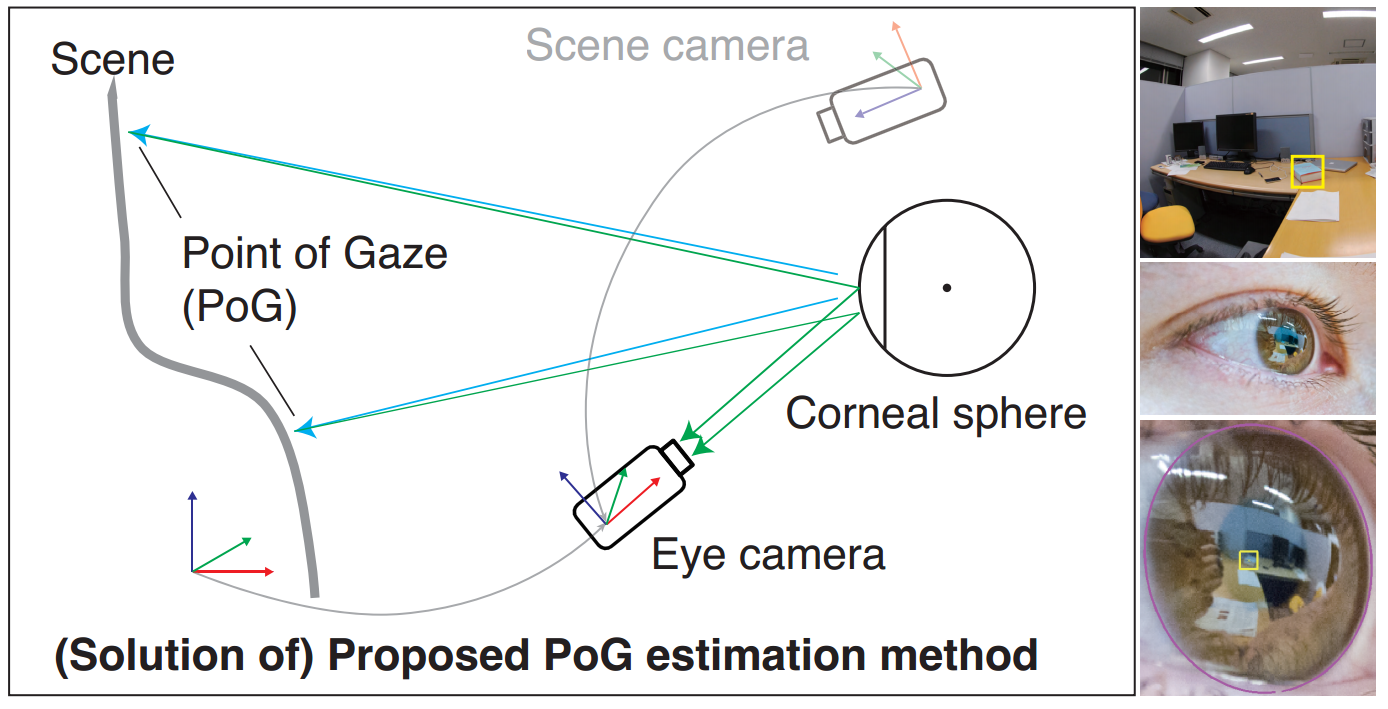
\includegraphics[width=4.5in,height=2.5in]{chrisitanN.png}
  \caption{Eye Gaze Tracking (EGT).}
  \label{christian}
\end{figure}

There is still room for further improvement over image quality. Therefore, authors have proposed that one could improve the corneal image through contrast enhancement, super-resolution, eye lash and iris removal or map the point of gaze into a high quality scene image, using passive correspondence matching between corneal and scene image.


\begin{figure}[!hbt]
  \centering
  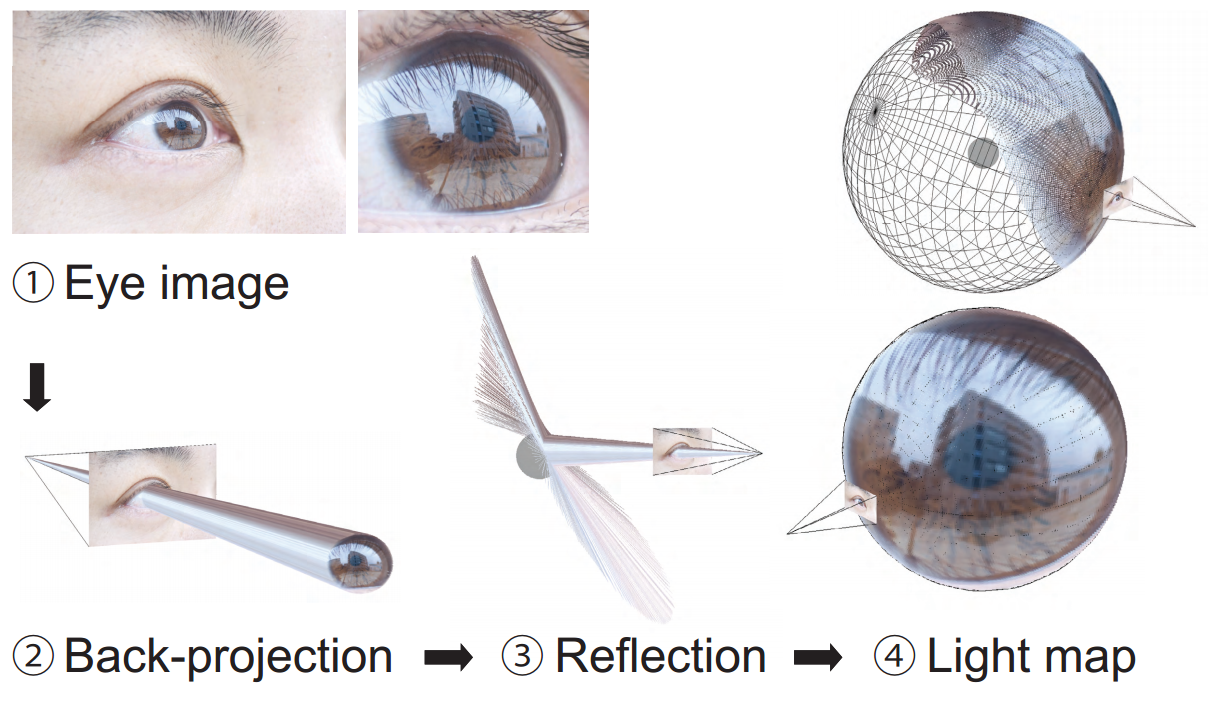
\includegraphics[width=4.5in,height=2.5in]{chrisitanN2.png}
  \caption{Corneal Reflection Model.}
  \label{christian}
\end{figure}


Hence, to summarize approaches in the paper, authors describe eye-gaze tracking as an important problem with a long history and various applications. However, state-ofthe-art geometric vision-based methods still lacks major functionalities. One is the requirement for calibration of a static relationship between eye camera and scene. Another is parallax error that occurs when the depth of the scene varies. Further, in this paper a novel concept is defined for eye-gaze tracking that solves limitations on using corneal imaging.\\

The prospective work will take advantage from the observations defined in the paper. The method is that cornea reflects the surrounding scene over a wide field of view and it is shown how to extract that information and determine the point of gaze directly in an eye image. This is of high usage in the prospective work of the thesis. To apply the solution, a closed-form solution is developed in the paper to obtain the gaze reflection point, where light from the point of gaze reflects at the corneal surface into a camera. In addition, quantitative and qualitative evaluation showen in the paper that this method results into considerable accuracy and successfully supports depth-varying environments.

\subsection{A Probabilistic Approach to Online Eye Gaze Tracking Without Explicit Personal Calibration}

In Jixu Chen, et.al \cite{21} paper, A Probabilistic Approach to Online Eye Gaze Tracking Without Explicit Personal Calibration, authors have proposed a new probabilistic gaze estimation framework. Gaze estimation in the proposed framework combines gaze prior with the 3D eye gaze model.

\begin{figure}[!hbt]
  \centering
  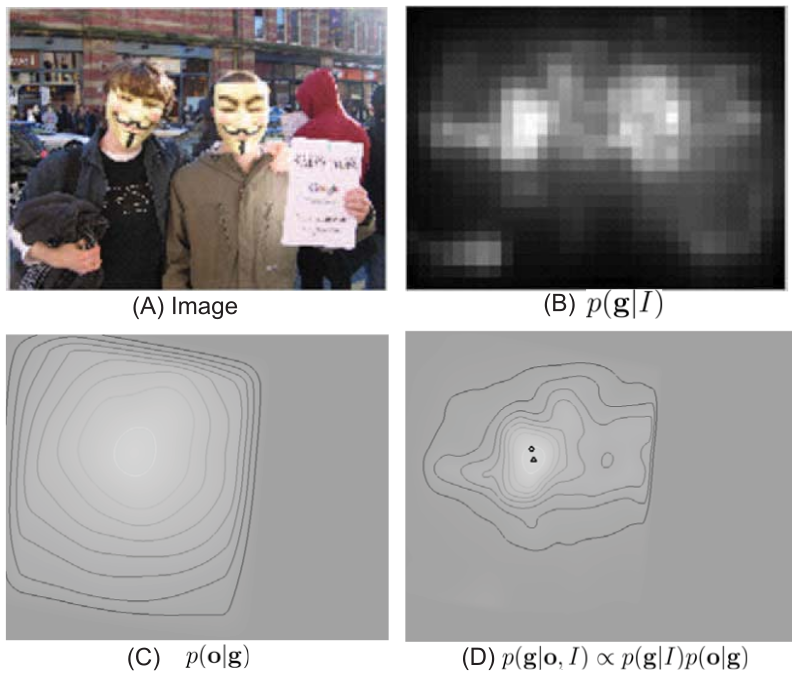
\includegraphics[width=4in,height=3.5in]{jixu.png}
  \caption{Probabilistic gaze estimation. (A) is the shown image. (B) is the saliency map $p(g|I)$ of the image. (C) is the gaze likelihood map given the optical axis. (D) is the gaze posterior probability map. The triangle shows the maximum posterior point. The circle shows the estimated gaze using the conventional method.}
  \label{jixu}
\end{figure}


\begin{figure}[!hbt]
  \centering
  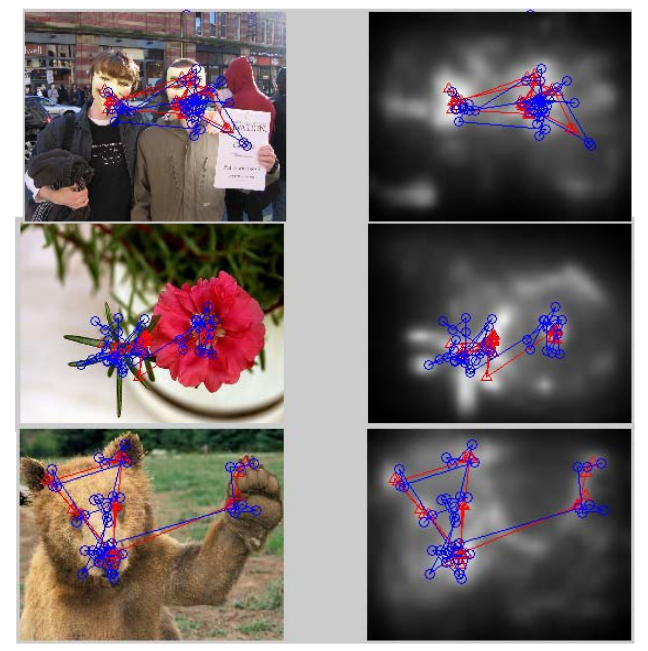
\includegraphics[width=4in,height=4in]{jixu2.png}
  \caption{An example of probabilistic gaze estimation result on three images. Red dots are the results of the proposed method. Blue dots are the results of the conventional method with 9-point calibration. The left column shows the gaze fixations superimposed on the original image, while the right column shows the fixations superimposed on the saliency map.}
  \label{jix2}
\end{figure}

The proposed approach eliminates the explicit personal calibration procedure compared to existing conventional gaze estimation methods. Subsequently, the proposed method changes the existing deterministic eye gaze tracking to probabilistic eye gaze tracking which allow to combine eye gaze prior with optical axis estimates. This simultaneously estimate 3D gaze point and the personal eye parameters in an incremental manner without any interruption from the user.


In the paper, authors compared the proposed approach with the most recent implicit personal calibration method. The proposed approach allows natural head movement and enable high gaze estimation accuracy of less than three degree which is better compare to current methods of 3.5 degrees accuracy as mentioned in the paper. The system also does not need any training data from the subject beforehand due to its novel incremental learning framework. The system quickly learns to the user actions and improves its performance gradually as the user uses the system. In order to improve the speed of the system, authors have further extended the system without computing the saliency map by assuming that the prior gaze distribution follows a Gaussian distribution with a mean located in the center of the screen.

Relating prospective work, this appraoch has limitations. The approach is limited in free-viewing scenarios when users are naturally viewing images or videos. Studies in visual attention have already shown that if the user is performing a specific visual task, his/her gaze distribution is driven by the task. The proposed gaze prior, either saliency map or Gaussian gaze prior, may not be applicable in this case.

\subsection{Interacting with the Computer using Gaze Gestures}

In Heiko Drewes, et.al \cite{22} paper, Interacting with the Computer using Gaze Gestures, authors review several noval approaches to direct computer by eye gaze. The work in the paper mainly focuses on eye motion in particular gaze gestures instead of using fixations and dwell times. Gaze gestures are robust to accuracy problems and flexible against calibration shift. Similar study described in the paper inidcates that complex gaze gestures are intentionally being performed by the users. Moreover, analysis on which kind of gestures occur by the user unintentionally during usual interaction with the computer. Further in the paper, experiments illustrates on the integeration of gaze gestures into working with standard desktop applications and interacting with different media devices.

\begin{figure}[!hbt]
  \centering
  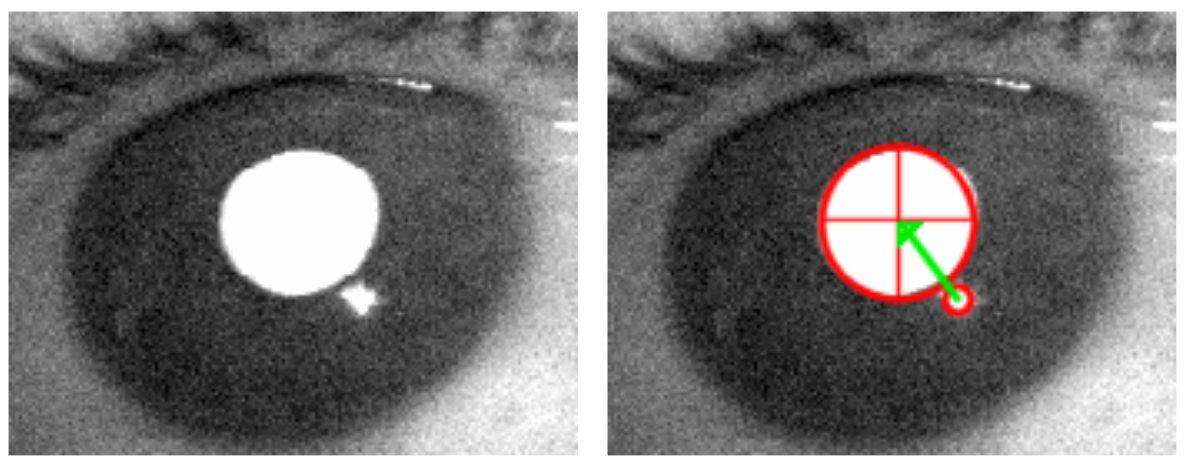
\includegraphics[width=4.5in,height=2in]{heiko.png}
  \caption{Video-based eye-tracking uses the reflection of an infrared LED and the center of the pupil to calculate the direction of the eye gaze. The reflection spot stays in the same position, while the pupil moves.}
  \label{heiko}
\end{figure}

The proposed algorithm in the paper is not fully researched therefore we will not at full extent use this approach in the prospective work. Authors indicated that further user studies needed to be done on the research of analyzing which gestures occur unintentional during normal user looking such as during watching videos. Optimnzation can be applied on the proposed algorithm where the objective functon includes grid size 's' and timeout 't' variables. Fewer unintended gestures can be obtain by using a bigger grid size of the dimensions of the display. The grid size affects gestures because eye movements normally stay within the display. Furthermore, typical saccade lengths are much smaller than the width or height of the display.



\section{Calibration Strategies}

The calibration is an individual process that has to be conducted for each user separately before using the eye tracker \cite{13}. The reason behind this is that the calibration includes human-specific parameters (such as cornea curvature and angle kappa) and geometric information (such as relative location and orientation between cameras). As we are using head-mounted device in our case, pupil positions are mapped into the scene video of a head-mounted device. The estimation method by itself is independent of the hardware approach. Interpolation-based methods typically create a 2D mapping from pupil to gaze positions. Various approaches exist to assess this mapping by polynomial functions \cite{26} or neural networks \cite{27}. Interpolation methods typically use linear or quadratic polynomial models to represent the mapping between image features and gaze. Calibration procedure determine unknown coefficients in the polynomial functions used in these models.\\

Another approach which can be used for calibration is smooth pursuit. It identify user gaze at moving objects, by correlating the user’s eye movement with the trajectory of the objects. Smooth pursuit is good in collecting gaze data only when the user actually attends, and this can be done iteratively \cite{4}. If a user is interrupted during the calibration, the procedure can resume and did not have to start all over again. Target velocity is also of importance. The velocity of a human smooth pursuit eye movements is limited to up to 30$^{\circ}$/s \cite{5}. Greater speed lead to catch-up eye movements. On the other hand, the detection rate for smooth pursuits also decreases when targets are too slow \cite{6}. The speed of the target also affects the duration of the calibration as if the target moves slowly, it will take longer to sample the output space. 

\subsection{Pursuit calibration: making gaze calibration less tedious and more flexible}

In Ken Pfeuffer, et.al \cite{4} paper, Pursuit calibration: making gaze calibration less tedious and more flexible, authors introduced pursuit calibration as a novel method for gaze calibration. The method mentioned in this paper is a relatively radical departure with respect to conventional approaches, because it calibrates eye gaze against a moving target and exploit smooth pursuit eye movement to determine when the user is following the target. 
\begin{figure}[!hbt]
  \centering
  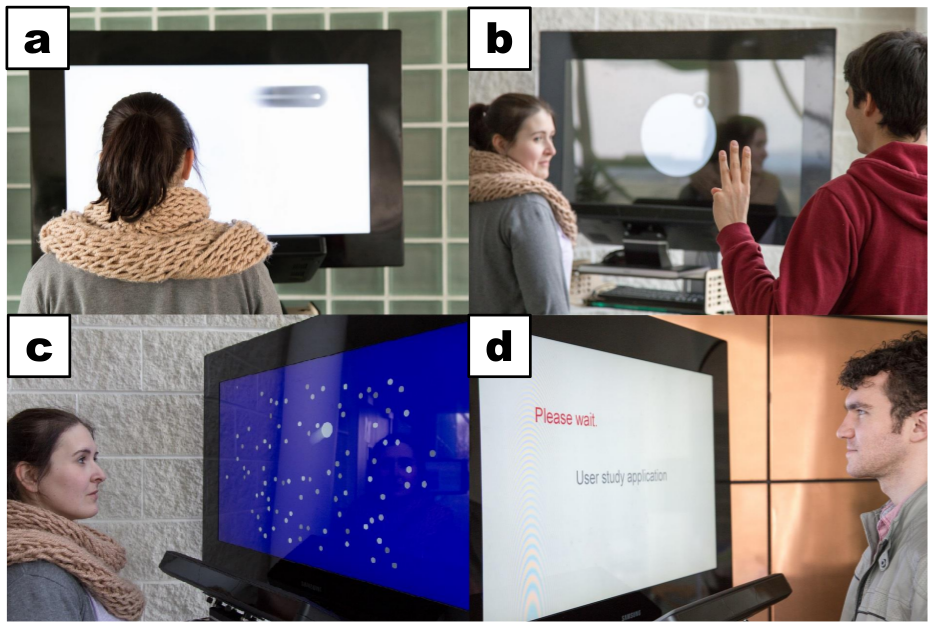
\includegraphics[width=4in,height=2.5in]{kenpfeffer.png}
  \caption{Pursuit calibration is based on moving targets (a), tolerates interruptions (b), can blend with application tasks (c) and calibrate users even when they are not aware (d).}
  \label{kenpfeffer}
\end{figure}

This leads to novel strategies for more intelligent sampling of calibration points, as well as usability advantages in tolerating user distraction and facilitating casual calibration. Pursuit calibration is simple in its core design but lends itself to implement gaze calibration in creative and innovative ways.\\

Regarding the prospective work, paper shows that in order for pursuit calibration to be integrated in the applications, it requires careful interface design. The accuracy study in the paper showed that a target that is too quick and therefore hard to follow for the eye. On the other hand, one that is too slow avoids detection of correlation.  Therefore, these finding are highly important for the prospective work, as we are going to higly focus on pursuit calibration in the prospective work.

\subsection{A Smooth Pursuit Calibration Technique}

In Feridun Mert Celebi, et.al \cite{17} paper, A Smooth Pursuit Calibration Technique, authors have discussed the potential trade-offs of smooth pursuit calibration over community standard 9-point-sparse calibration. They have illustrated that the choice of the calibration routine should be made based on the needs of the experimenter. However, for smoothing distortions in the eye tracking data a collection of up to 1600 data points provides greater flexibility. It also might be the case to increase spatial noise. It has been evidenced by the data provided in the paper that smooth pursuit calibration delivers several improvements to the accuracy and stability of the data. This data, however, is indexed by defined mean errors and standard deviations. These improvements have become even more important to address because participants are allowed to move their heads freely. However, it is assumed that the need for stability in the use of desktop-mounted systems is increased.\\

Furthermore, additional insight about the participants mentioned in the paper can be found by examining the properties of smooth pursuit in subjects participating in experimental studies. As an example, previous studies have shown that the smooth pursuit properties such as gain and alg are associated with neuropsychiatric conditions. Smooth pursuit properties also shows robust psychometric properties which are most likely related to attentional control. Individual differences and systematic deviations from POR expectations may provide a new and exciting area for future clinical and technical advancement after examining the interplay between these smooth pursuit properties.\\

As the findings from the paper gives a comprehensive overview of potential trade-offs of smooth pursuit calibration for 9-point-sparse calibration, it is clearly important for our prospective work on calibration method. The different choice of calibration strategies and their pitfalls mentioned in the paper help alot to decide which ones can perform better than others under which conditions.

\subsection{Orbits: Gaze Interaction for Smart Watches using Smooth Pursuit Eye Movements}

In Augusto Esteves, et.al \cite{18} \cite{19} papers on Orbits: Gaze Interaction for Smart Watches using Smooth Pursuit Eye Movements, authors have described that their work enable hands-free interaction on smart watches, but they have also included the possibility and wherabouts of combination of Orbits with other modalities. As it has been examplify in the paper that Orbits can be added as a complementary modality when user's hands are engaged in other activities such as cooking etc,. In cases other than smart watches where hand interaction is difficult, such as using a smartphone on a treadmill, orbits can be used easily.

\begin{figure}[!hbt]
  \centering
  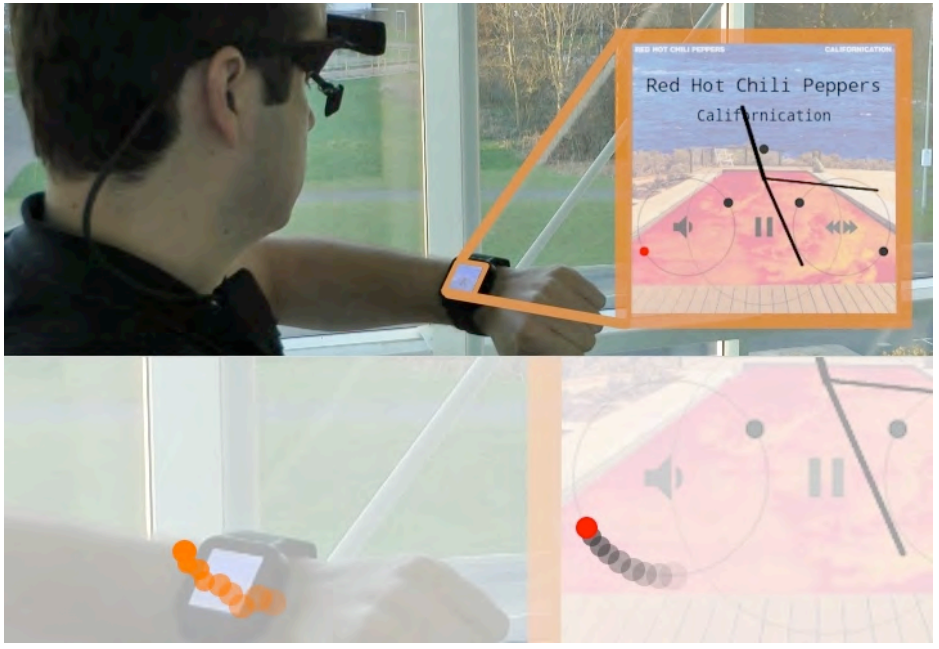
\includegraphics[width=4in,height=2.5in]{augusto.png}
  \caption{Top: a user raises the volume of his smart watch music player using Orbits gaze input controls. The UI shows the volume, pause/play and previous/next controls with orbiting targets for gaze selection. Bottom: how Orbits enables gaze input on smart watches. The technique can robustly detect which of the controls is actively being followed by correlating each Orbits’ target with the user’s gaze.}
  \label{augusto}
\end{figure}

Orbits can be used in cases where its sometimes impossible to do hand interaction such as assistive interfaces. Therefore, in the prospective work orbits can give solution to handle similar difficult situations. The reason why orbits are so successfull in dealing with such situations is because it uses the relative movement of the eyes, and it does not need any registration between the user’s gaze and the watch’s coordinate systems. Therefore, the need of scene cameras in head-worn eye trackers will not longer be needed. This further introduce privacy concerns. Hence, It can be said that orbits can potentially be used with EOG (electrooculography) based trackers, which monitor eye movements through the electrical signal generated by them.


\subsection{Orbits: Enabling Gaze Interaction in Smart Watches Using Moving Targets}

In a similar paper \cite{19}, Orbits: Enabling Gaze Interaction in Smart Watches Using Moving Targets, authors introduced Orbits which as described in the paper is a novel interaction technique for smart watches that relies not on touch, but in gaze input. Authors in the paper, illustrated three main example applications that show how users can take advantages from interfaces which combine movement and gaze controls. The main focus of this paper is on moving targets with smart watches.

Authors mentioned in the paper that Orbits interfaces can be used in car dashboards exercise equipment such as rowing machines, treadmills, ubiquitous environments such as lighting and entertainment systems. Orbits can also be used in novel and more robust assistive interfaces. Furthermore, this method can also be applied to interface with real world. It can be done by detecting and reacting to naturally occurring movements in the environment for example the London Eye, and digital billboards. Overall, Orbits gives an insight to how we will be able to interact with the devices of the future, a future where touch is not core to the experience, but complimentary to other modalities such as a gaze.

\subsection{Pursuits: Eye-based interaction with moving targets}

In Melodie Vidal, et.al \cite{6} paper, Pursuits: Eye-based interaction with moving targets, authors have presented a pursuit method for natural eye-based interaction with moving objects. This method as introduced in the paper, describes a new tracking principle which solves the need for accurate calibration of gaze direction and mapped this problem as a matching of eye and object movement. Authors have described three applications in this paper which show that the Pursuits method is natural and effective for selection of moving targets, and allows to embrace movement in user interfaces in innovative ways. 

\begin{figure}[!hbt]
  \centering
  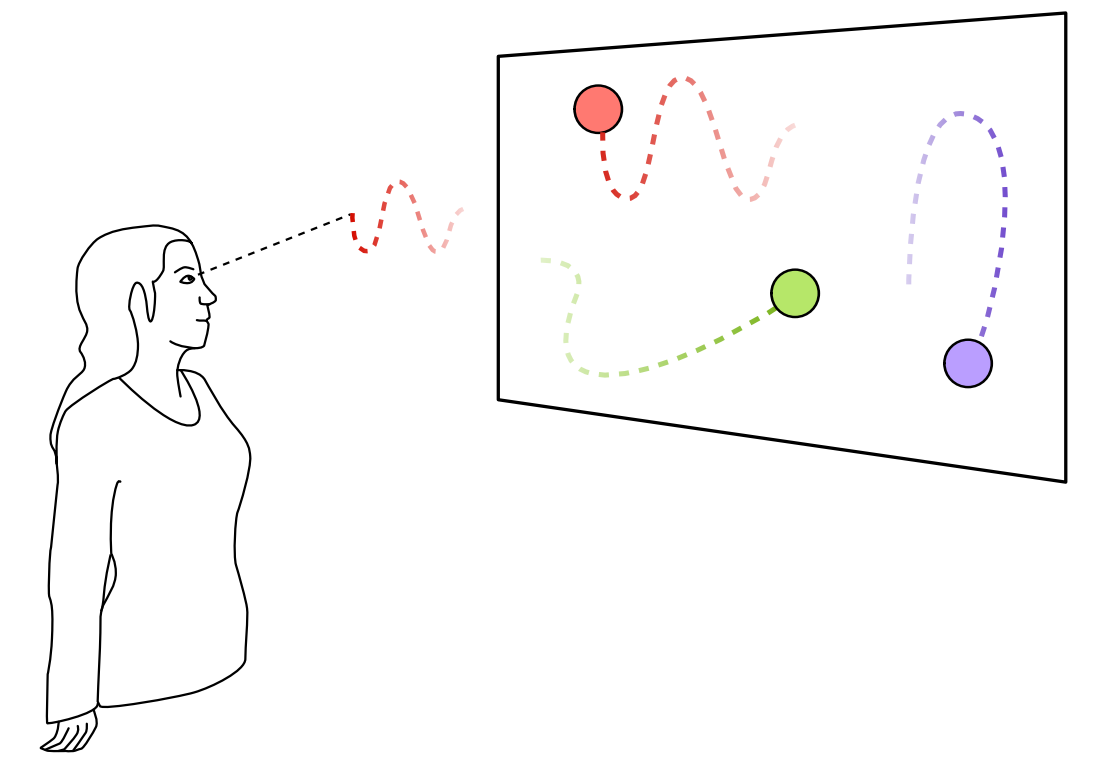
\includegraphics[width=4in,height=2.5in]{melodie.png}
  \caption{When a user follows a moving object on the screen, her eyes perform the same trajectory as the followed object’s.}
  \label{melodie}
\end{figure}

Pursuits, the proposed method in paper, enable new perspectives which would help to look at design and implementation of eye-based interfaces, and shifting the emphasis from gaze estimation to movement analysis. It could also shift the emphasis from fixations to other activity of our eyes, and from interaction with static interfaces to interaction with dynamic content.\\

\begin{figure}[!hbt]
  \centering
  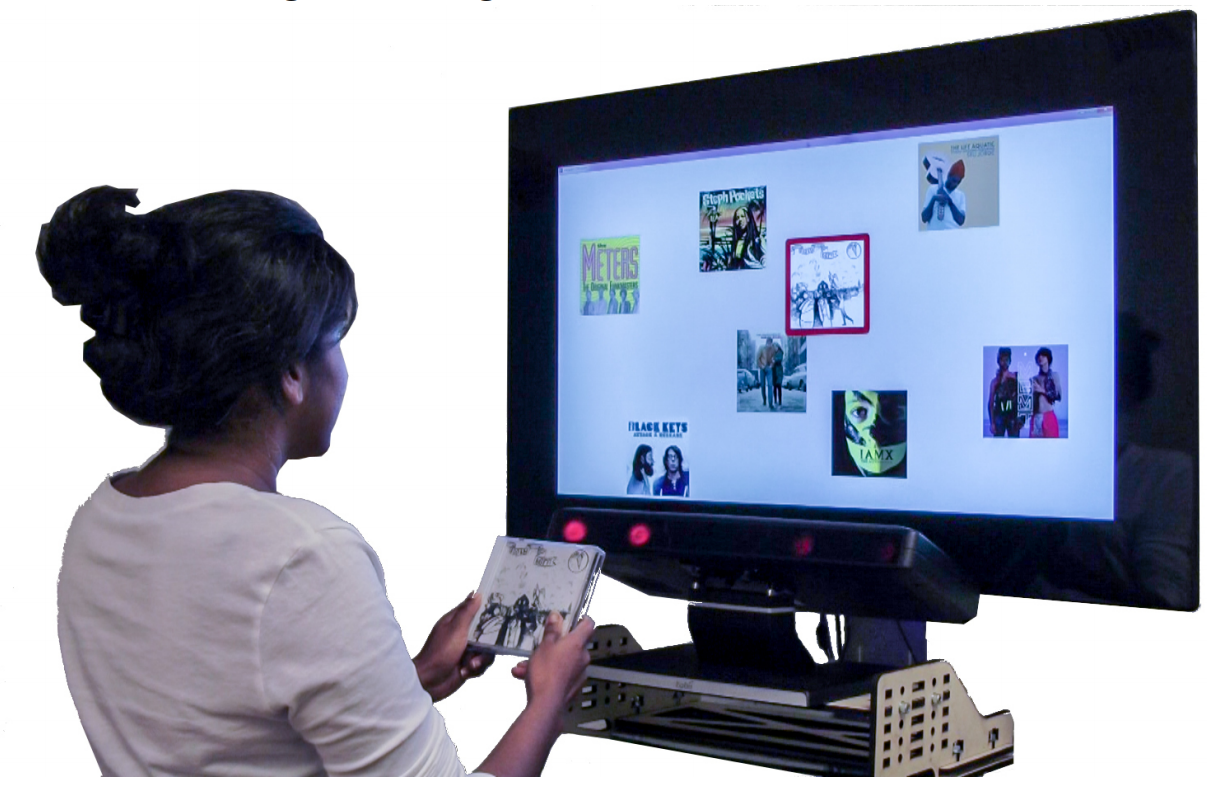
\includegraphics[width=4in,height=2.5in]{melodie2.png}
  \caption{A user is interested in listening to a music album. She walks up to the in-store display, locates the album on the screen and follows its movement with her eyes. A sample of the music starts to play automatically.}
  \label{melodie2}
\end{figure}

In the prospective work eye-based interaction will be used as an estimation of eye gaze direction. Authors have introduce Pursuits and illustrate it as a novel and very different eye tracking method. It is based on following the trajectory of eye movement and comparing this with trajectories of objects in the field of view. As the eyes naturally follow the trajectory of moving objects of interest, the method described in the paper is able to detect what the user is looking at, by matching eye movement and object movement. Authors presented Pursuits with three applications that demonstrate how the method support natural interaction with moving targets.

\subsection{Remote Point-of-gaze Estimation With Single-point Personal Calibration Based On The Pupil Boundary And Corneal Reflections}

In Elias D. Guestrin, et.al \cite{23} paper, Remote Point-of-gaze Estimation With Single-point Personal Calibration Based On The Pupil Boundary And Corneal Reflections, authors have proposed a new method for non-contact point-of-gaze (PoG) esitmation which is remote based and robust against head movements. This new approach requires user to do a simple personal calibration procedure by fixating on a single calibration point. The method also uses the pupil boundary and at least two corneal reflections which are described as virtual images of light sources in the paper. These corneal reflections are being extracted from eye images captured by at least two video cameras. Results from a prototype system showed root mean square point of gaze estimation errors of approx. 0.4-0.6$^{\circ}$ of visual angle. This kind of accuracy is as good as the best commercially available systems which use multiple-point personal calibration procedures. Furthermore, its much better than any other system that use a single-point personal calibration procedure.

\begin{figure}[!hbt]
  \centering
  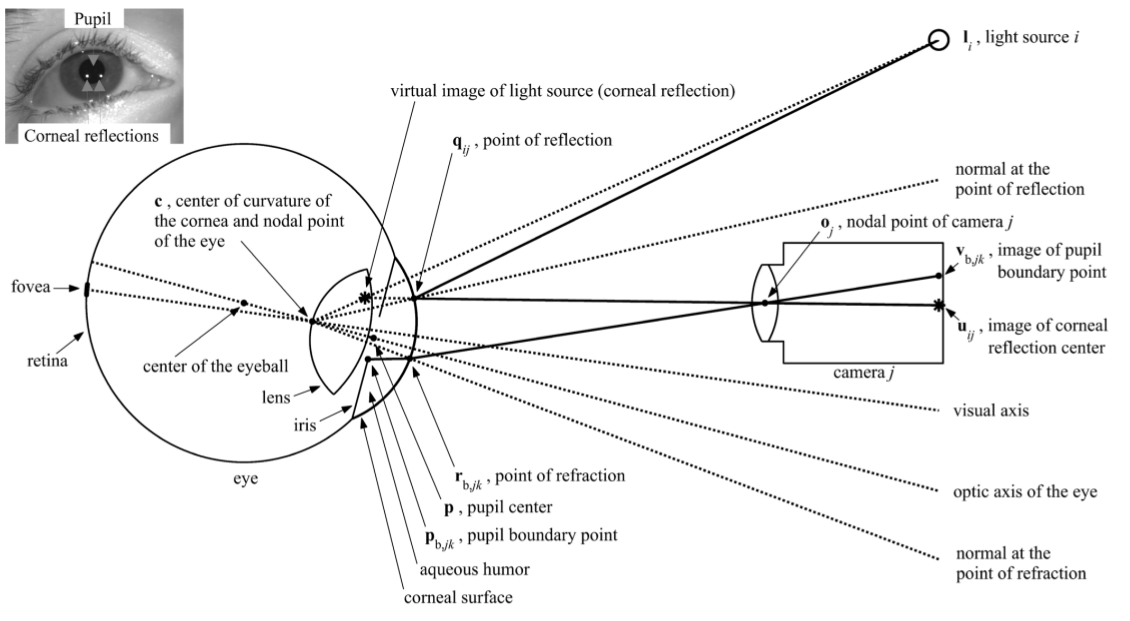
\includegraphics[width=4.5in,height=2.5in]{elias.png}
  \caption{Ray-tracing diagram (not to scale in order to be able to show all the elements of interest), showing schematic representations of an eye, a camera and a light source. Inset: eye image indicating the pupil and two corneal reflections.}
  \label{elias}
\end{figure}


As the prospective will be on calibration procedures, the results from the papers show that the proposed method makes it possible to evaluate the point of gaze with an accuracy of 0.4-0.6$^{\circ}$ of visual angle after completing a single-point personal calibration procedure. Because kind of accuracy is comparable or better with current systems, the approach in the paper surpass current methods and show great results compare to the previously described methods in the literature and are related to the prospective work.

\newpage

\section{Observations}

Following are the observations identified from a long-term gaze dataset \cite{28} that contains full-day recordings of natural visual behaviour of 10 participants (more than 80 hours in total). This dataset includes annotations for eight sample activity classes (outdoor, social interaction, focused work, travel, reading, computer work, watching media, eating) and periods with no specific activity. Observations are also deduced from other pupil data recordings in real world roaming enivronment. These observations are related to the papers findings as mentioned in previous sections.\\

\begin{figure}[!hbt]
  \begin{subfigure}{.5\textwidth}
    \centering
    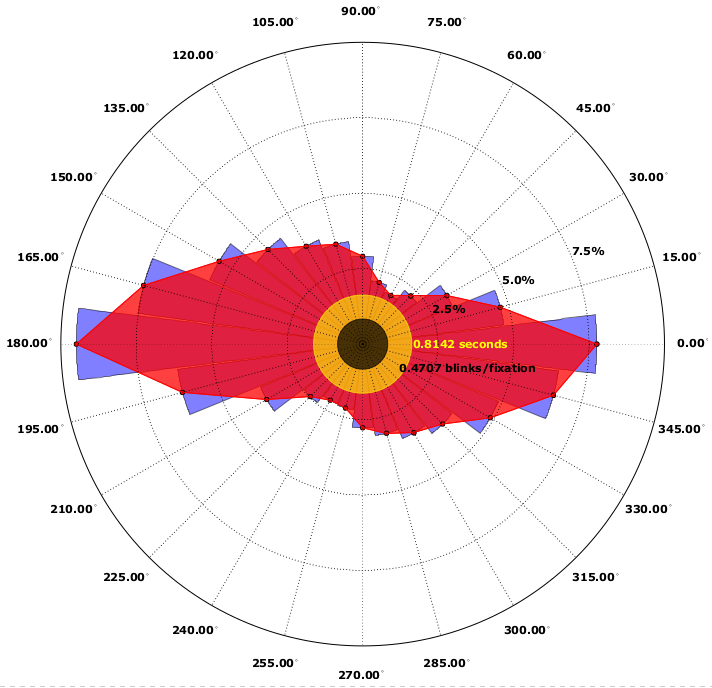
\includegraphics[width=2.5in,height=2.5in]{obs1.png}
    \caption{Reading}
    \label{obs1}
  \end{subfigure}
  \begin{subfigure}{.5\textwidth}
    \centering
    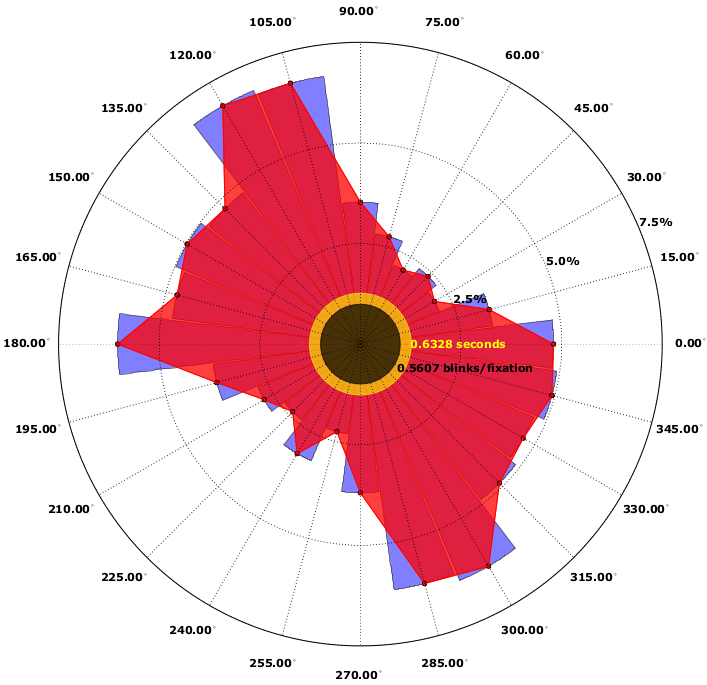
\includegraphics[width=2.5in,height=2.5in]{obs2.png}
    \caption{Watching media}
    \label{obs2}
  \end{subfigure}
  \caption{Sample saccade direction distributions for "reading" and "watching media" for participant 6.}
\end{figure}


Most of the participants were students and wore the eye tracker through one day of their normal university life. Participant's activities differ across days, their overall daily routines were still almost similar. However, full-day recordings of multiple particiants has a large variability with respect to the number, type, and distribution of activities that the participants performed. Therefore, the best performing saccade encoding, eye movement characteristics, is highly dependent on the participant and can be seen in the Figure \ref{obs3}.\\ 

\begin{figure}[!hbt]
  \centering
  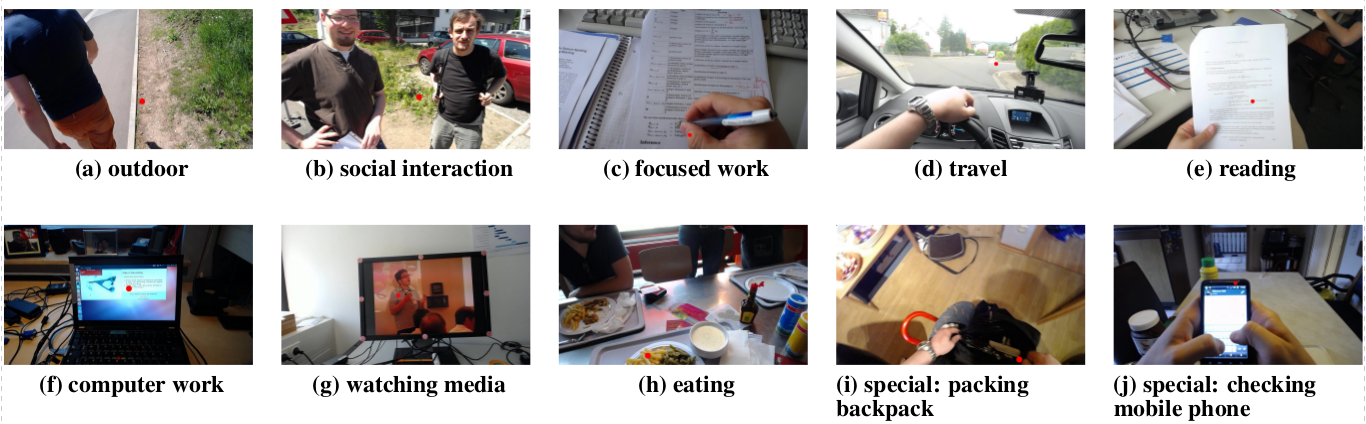
\includegraphics[width=5in,height=2in]{obs3.png}
  \caption{Sample scene images for each activity class annotated in the dataset showing the considerable variability in terms of place and time of recording. The red dot indicates the gaze location in that particular image.}
  \label{obs3}
\end{figure}

Following are the main three observations of anohter pupil data recordings:

1. Eye does pursuit movement on moving objects but does not follow it too long. However, it could be depended on users interest on the object.\\

2. Eye movement verses head movement to pursue moving object is highly correlated on how far the object is moving from user's point of view. If the object is far, head movement is more likely to occur than eye movement and vice versa.\\

3. If a person is nearby of moving object, its more likely that head movement occur to follow the moving object.\\




% \clearpage
% \begingroup
%   \pagestyle{plain}
%   \bibliographystyle{acm_adjusted}
%    \phantomsection
% 	\addcontentsline{toc}{section}{Bibliography}
% 	\bibliography{references}\emph{}	
% 	\vfill
%   \clearpage
% \endgroup 

  \newpage

  \begin{thebibliography}{00}
  \bibitem{1}  Guestrin, E., and Einzenmann, M. General theory of remote gaze estimation using the pupil center and corneal reflections. In IEEE Trans. on Biomedical Engineering, vol. 53 (2006), 1124–1133.
  \bibitem{2} CA. Duchowski,Eye Tracking Methodology: Theory and Practice.Springer-Verlag, 2003.
  \bibitem{3} Eye Tracking and Head Movement Detection: A State-of-Art Survey Amer Al-Rahayfeh and Miad Faezipour
  \bibitem{4} Ken Pfeuffer , Melodie Vidal , Jayson Turner , Andreas Bulling , Hans Gellersen, Pursuit calibration: making gaze calibration less tedious and more flexible, Proceedings of the 26th annual ACM symposium on User interface software and technology, October 08-11, 2013, St. Andrews, Scotland, United Kingdom.
  \bibitem{5} Young, L., and Sheena, D. Survey of eye movement recording methods. Behavior Research Methods and Instrumentation 7 (1975),397–429.
  \bibitem{6} Vidal, M., Pfeuffer, K., Bulling, A., and Gellersen, H. Pursuits: Eye-based interaction with moving targets. In Proc. of CHI EA ’13, ACM (2013).
  \bibitem{7} Satoh K., Uchiyama S., and Yamamoto H., “A head tracking method using birD's-eye view camera and gyroscope,” in Proc. 3rd IEEE/ACM ISMAR, Nov. 2004, pp. 202–211.
  \bibitem{8} Coetzer R. C. and Hancke G. P., “Eye detection for a real-time vehicle driver fatigue monitoring system,” in Proc. IEEE Intell. Veh. Symp., Jun. 2011, pp. 66–71.
  \bibitem{9} Gips J., DiMattia P., Curran F. X., and Olivieri P., “Using EagleEyes—An electrodes based device for controlling the computer with your eyes to help people with special needs,” in Proc. Interdisciplinary Aspects Comput. Help. People Special Needs, 1996, pp. 77–84.
  \bibitem{10} Gneo, Massimo; Schmid, Maurizio; Conforto, Silvia; D’Alessio, Tommaso (2012). A free geometry model-independent neural eye-gaze tracking system. Journal of NeuroEngineering and Rehabilitation. 
  \bibitem{11} Miluzzo, E., Wang, T., Campbell, A.T., 2010. EyePhone: activating mobile phones with your eyes. In: Proceedings of the Second ACM SIGCOMM Workshop on Networking.
  \bibitem{12} Pino, C., Kavasidis, I., 2012. Improving mobile device interaction by eye tracking analysis. In: 2012 Federated Conference on Computer Science and Information Systems (FedCSIS). pp. 1199-1202.
  \bibitem{13} hEYEbrid: A Hybrid Approach for Mobile Calibration-free Gaze Estimation, Christian Lander, Markus Loechtefeld, Antonio Krueger
  \bibitem{14} He, J., Fields, B., Peng, J., Cielocha, S., Coltea, J., Roberson, S., 2013. Fatigue detection using smartphones. In: International Conference on Psychology and Applications, Beijing, China.
  \bibitem{15} Eye gaze tracking techniques for interactive applications, Carlos H. Morimoto , Marcio R.M. Mimica.
  \bibitem{16} In the Eye of the Beholder: A Survey of Models for Eyes and Gaze. Dan Witzner Hansen, Member, IEEE, and Qiang Ji, Senior Member, IEEE
  \bibitem{17} A Smooth Pursuit Calibration Technique, Feridun  Mert  Celebi, Elizabeth S.  Kim, Carla  Anne  Wall, Frederick Shic.
  \bibitem{18} Orbits: Gaze Interaction for Smart Watches using Smooth Pursuit Eye Movements, Augusto Esteves, Eduardo Velloso, Andreas Bulling, Hans Gellersen
 \bibitem{19} Orbits: Enabling Gaze Interaction in Smart Watches Using Moving Targets, Augusto Esteves, Eduardo Velloso, Andreas Bulling, Hans Gellersen
 \bibitem{20} I see what you see: Point of Gaze Estimation from Corneal Images, Christian Nitschke, Atsushi Nakazawa, and Toyoaki Nishida
 \bibitem{21} Jixu Chen and Qiang Ji. 2011. Probabilistic Gaze Estimation Without Active Personal Calibration. In Proceedings of the 2011 IEEE Conference on Computer Vision and Pattern Recognition (CVPR '11).
 \bibitem{22} Drewes, H., and Schmidt, A. Interacting with the computer using gaze gestures. In Proc. of INTERACT '07, Springer (2007)
 \bibitem{23} Elias D. Guestrin, and Moshe Eizenman Remote Point-of-gaze Estimation With Single-point Personal Calibration Based On The Pupil Boundary And Corneal Reflections
 \bibitem{24} Poole, A., Ball, L.J., 2005. Eye tracking in human-computer interaction and usability research: current status and future prospects. In: Ghaoui, C. (Ed.), Encyclopedia of Human Computer Interaction.
 \bibitem{25} David A. Robinson. 1963. A Method of Measuring Eye Movement Using a Scleral Search Coil in a Magnetic Field. IEEE Transactions on Bio-medical Electronics 10 (1963), 137–45. https://doi.org/10.1109/TBMEL.1963.4322822
 \bibitem{26} Juan J. Cerrolaza, Arantxa Villanueva, and Rafael Cabeza. 2012. Study of Polynomial Mapping Functions in Video-Oculography Eye
Trackers. ACM Trans. Comput.-Hum. Interact. 19, 2, Article 10 (July 2012), 25 pages. https://doi.org/10.1145/2240156.2240158
 \bibitem{27} Qiang Ji and Xiaojie Yang. 2002. Real-Time Eye, Gaze, and Face Pose Tracking for Monitoring Driver Vigilance. Real-Time Imaging (2002), 357–377. https://doi.org/10.1006/rtim.2002.0279
 \bibitem{28} Julian Steil , Andreas Bulling, Discovery of everyday human activities from long-term visual behaviour using topic models, Proceedings of the 2015 ACM International Joint Conference on Pervasive and Ubiquitous Computing, September 07-11, 2015, Osaka, Japan 
 \bibitem{29} https://www.pupil-labs.com/
  \end{thebibliography}


\end{document}